\documentclass{article}
\usepackage[authoryear]{natbib}
% \usepackage[numbers]{natbib}
\usepackage[final]{neurips_2023}
\usepackage[utf8]{inputenc} % allow utf-8 input
\usepackage[T1]{fontenc}    % use 8-bit T1 fonts
\usepackage{hyperref}       % hyperlinks
\usepackage{url}            % simple URL typesetting
\usepackage{booktabs}       % professional-quality tables
\usepackage{amsfonts}       % blackboard math symbols
\usepackage{nicefrac}       % compact symbols for 1/2, etc.
\usepackage{microtype}      % microtypography
\usepackage{xcolor}         % colors
\usepackage{graphicx}       % images
\usepackage{footnote}       % footnotes
\usepackage{subcaption}

\title{Comparasion of ResNet50 and 3-layer Neural Network for Bird Identification}

\author{
  Wentai Ye\\
  Department of Engineering Technology\\
  KU Leuven\\
  \texttt{yewentai126@gmail.com} \\
  \And
  Joren Mangelschots \\
  Department of Engineering Technology\\
  KU Leuven\\
  \texttt{joren.mangelschots@student.kuleuven.be} \\
}
\usepackage{amsmath}

\begin{document}

\maketitle

\begin{abstract}
  Because of the decreasing biodiversity in nature reserves, we tought to manage this biodiverisity it would be nice to have a classificaiton system. With this classificaiton system we would be able to use images to recognise which species of birds are in the image. We used a baseline and an advanced ResNet50 neural network for the classification. 
\end{abstract}

\section{Introduction}

In the realm of environmental conservation and biodiversity research, the development of a machine learning algorithm capable of accurately classifying bird species from images represents a groundbreaking advancement. This technological endeavor addresses a critical challenge with far-reaching implications in various fields. 

The cornerstone of this project is its potential impact on conservation and biodiversity monitoring. Birds are often considered key indicators of an ecosystem's health. Therefore, the ability to automatically identify bird species is an invaluable asset for conservationists. This capability is particularly crucial in conservation areas, where monitoring the presence and diversity of bird species can yield vital information about the state of biodiversity and the effectiveness of ongoing conservation efforts.

Another significant aspect of this project is the efficiency and scalability it offers. Traditionally, the identification of bird species has been reliant on expert knowledge, a process that is both time-intensive and limited in scope. An automated system, on the other hand, can rapidly process a large volume of images, thereby facilitating the monitoring of more extensive areas and a greater variety of species than what is currently possible through manual methods.

Beyond its scientific and conservation applications, this tool also holds promise for public engagement and education. By integrating an automated bird identification system into apps and platforms used by bird watchers and nature enthusiasts, it can enhance their experience and knowledge. This, in turn, helps in raising public awareness about various bird species and broader conservation issues.

The input to our algorithm is an image. We then use a neural network to output a predicted bird species.
\section{Related Work}
Recent studies in bird species classification have explored various methodologies. \citet{haobin_fine-grained_2018} introduced a low-dimensional bilinear model that prioritizes computational efficiency by reducing feature dimensionality. \citet{zhang_improvements_2023} focused on improving the ShuffleNetV2 model, offering a lightweight yet effective solution suitable for resource-limited environments. \citet{vo_bird_2023} employed a YOLO-based framework, emphasizing real-time processing capabilities. \citet{zahra_el_bouni_bird_2021} utilized wavelet transform for feature extraction, showcasing effectiveness in handling varying textures and patterns. Lastly, \citet{budiman_classification_2022} adopted a K-Nearest Neighbors approach, highlighting simplicity and ease of implementation. 
\section{Dataset and Features}
1. Include a citation on where you obtained your dataset from. 
2. Describe your dataset: how many training/validation/test examples do you have? 
3. Depending on available space, show some examples from your dataset. Try to include examples of your data in the report (e.g. include an image, show a waveform, etc.).
4. What is the resolution of your images? 
5. Is there any preprocessing you did? 
6. What about normalization or standardization? 

The dataset in this study encompasses 525 bird species, featuring 84,635 training images, along with 2,625 images each for testing and validation (5 per species). Rigorous dataset analysis tools were applied to eliminate duplicates and low-quality images, ensuring the dataset's integrity and preventing leakage across train, test, and validation sets.\footnote{Laszewski, G. von. (2023). 100 Bird Species [Data set]. Kaggle. \url{https://www.kaggle.com/datasets/gpiosenka/100-bird-species}}

Each 224x224x3 color image in JPG format, predominantly featuring the bird, is meticulously categorized into 525 folders per species. Accompanying this is a comprehensive CSV file detailing file paths, labels, scientific names, dataset types, and class indices. 
The test and validation images, carefully chosen for their quality, enhance the dataset's robustness. 

The birds in each of the images will take up at least 50\% of the pixels in the image. The images are all gathered from the internet, they where thoroughly chekced for the presence of any duplicated data. This prevent the same images being in the test, validation and train set. 

There is one downside of the dataset, which is the ratio of male species to female species. The dataset contains of around 80\% of male images while only just containing 20\% female images. There is a good reason for it, being that male birds are far more colored, while the female birds are more bland. This makes that the algorithm will be good for detecting the male species but it will struggle giving a accurate classification for the female, because their coloring is more bland. 

For the Neural networks the images where augmented by also including the vertically swapped version of each image. 

\begin{figure}[h]
    \centering
    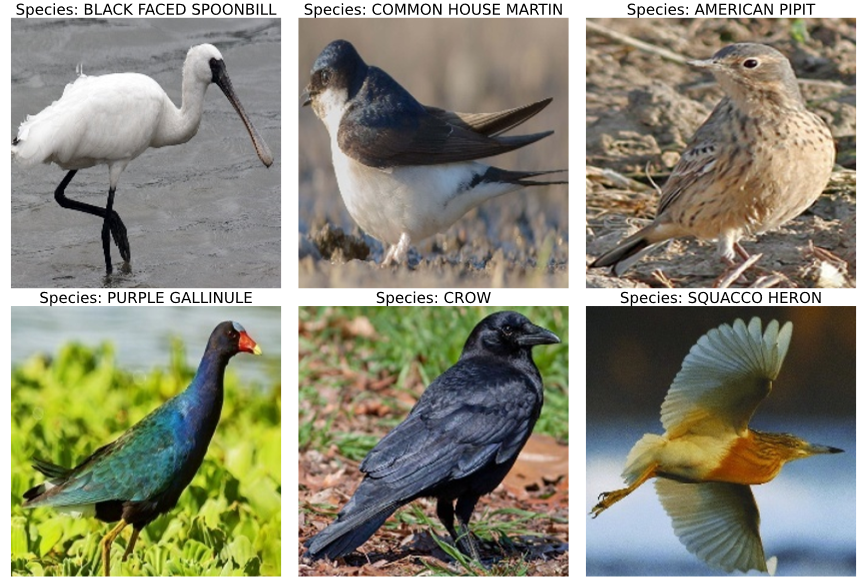
\includegraphics[width=0.5\textwidth]{figs/dataset.png}
    \caption{Images in dataset}
    \label{fig:dataset}
\end{figure}
\section{Methods}
\subsection{Neural network}
The first model is a model from the one of the exercise sessions about multiclass-classificication neural networks. The architecture of the model is a feedforward neural network with multiple densely connected layers. Each layer contains of a number of neurons which are decreasing progressively. The output layer has a number of neurons equal to the number of classes.

The learning in this model is done through backpropagation. This involves iteratively adjusting the weights of the connections based on the error of the prediction. The objective is to find the optimal weights that minimize the cross-entropy loss between the predicted probabilities and the true class labels. Because of timing issues, the training of the first model is done on a smaller set of 50 of the 525 classes. 

The first model was the model of the exercise session with 3 layers. In these layers the amount of neurons was changed to confirm with the amount of classes at the output layers, and the layers above have a higher number of nodes. The basic neural network model consist of two layers of 64 neurons and one layer of 50 neurons according to the figure \ref{fig:NN with 3 layers}. The improved neural network has 8 layers going down from 1024 neurons to 50 neurons, according to the figure \ref{fig:NN with 8 layers}

The basic neural network model is a model consisisting of a input layer which takes in the data type being (32, 32, 3) because the images are decreased in quality to improve the training. All the connected layers different from the output layer are fully connected layers with RELU activation,  this introduces non-linearity into the neural network. This activation makes the computation more efficient because it just involves a simple threshold at 0, which is way less computational hard then other activation systems. It is given by the following formula:

\[
\text{ReLU}(x) = \begin{cases}
    x & \text{if } x > 0 \\
    0 & \text{if } x \leq 0
\end{cases}
\]

The activation in the output layer is softmax, this transforms a vector of numbers into a probability distribution. It makes sure that the output values are between 0 and 1 and it sums to 1, this makes it possible for representing the probabilities. It is used together with cross-entropy loss. It measures the difference between the predicted probabilities and the true distribution of the labels. It is given by the following formula: 

\[\text{softmax}(\mathbf{x})_i = \frac{e^{x_i}}{\sum_{j=1}^{N} e^{x_j}}\]

Both of those neural network models are trained with a learning rate of 0.001. This value determines the stepsize at each iteration, while moving towards a minimum of the loss function. If the learning rate is big this can lead to an overshooting of the minimum and a failure to converge. When the learning rate is too small the convergence will happen really slowly. 

\begin{figure}[h]
    \centering
    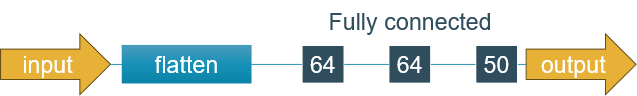
\includegraphics[width=0.5\textwidth]{figs/basic nn.png}
    \caption{NN with 3 connected layers architecture}
    \label{fig:NN with 3 layers}
\end{figure}

\begin{figure}[h]
    \centering
    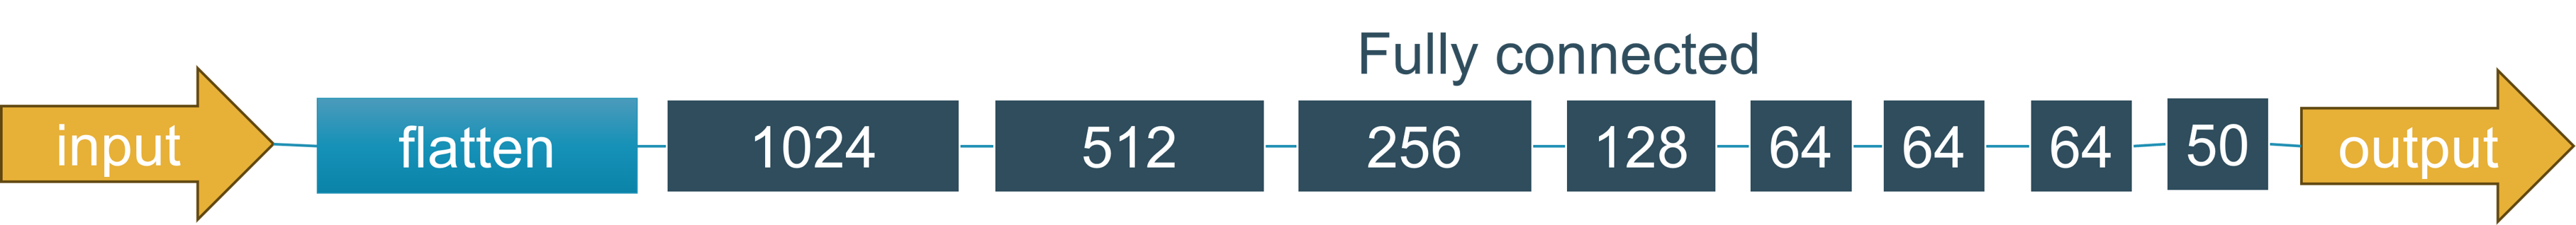
\includegraphics[width=0.5\textwidth]{figs/improved NN.png}
    \caption{NN with 8 connected layers architecture}
    \label{fig:NN with 8 layers}
\end{figure}

\subsection{ResNet}
ResNet, short for Residual Network, is a type of neural network architecture that was designed to enable the training of much deeper networks than was previously feasible. Introduced by Microsoft researchers in 2015, ResNet quickly became famous for its effectiveness, especially in image classification tasks. \citet{he_deep_2016} The ResNet architecture is composed of a series of residual blocks, which are composed of a series of convolutional layers. 

\begin{figure}[h]
    \centering
    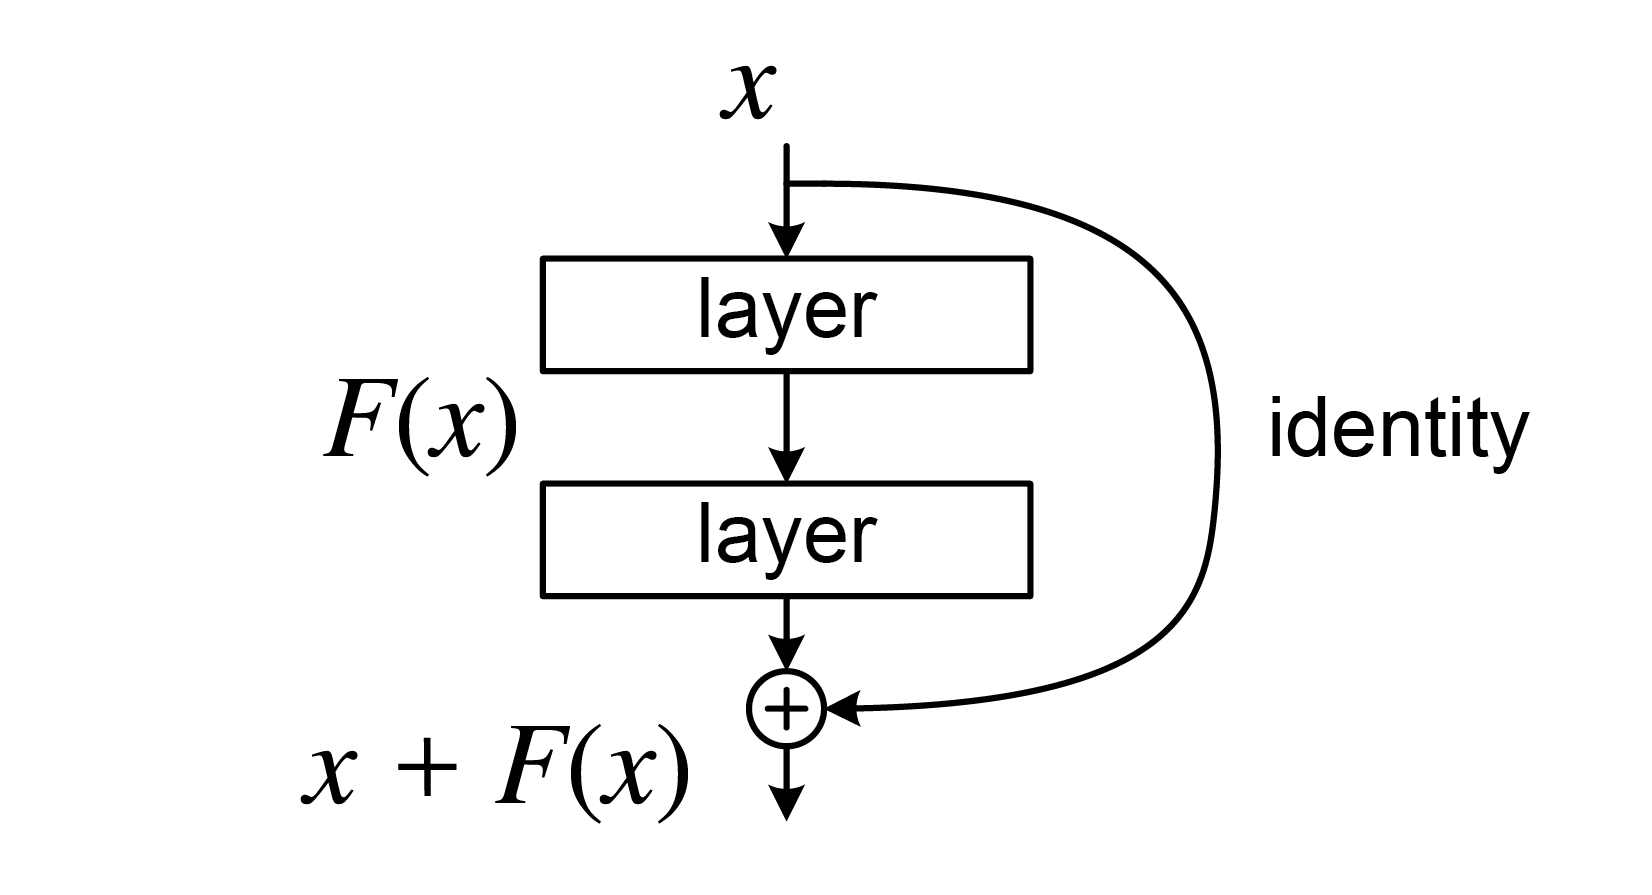
\includegraphics[width=0.5\textwidth]{figs/ResBlock.png}
    \caption{ResNet architecture}
    \label{fig:resnet}
\end{figure}

The ResNet (Residual Network) architecture, as illustrated in Figure \ref{fig:resnet}, represents a significant advancement in deep neural networks. This architecture is primarily characterized by its residual blocks and skip connections. The structure of ResNet can be described as follows:

\begin{itemize}
    \item \textbf{Residual Blocks:} Each residual block in ResNet is composed of several convolutional layers. These layers are designed to learn the residual functions with reference to the layer inputs. A typical residual block contains two or three convolutional layers.

    \item \textbf{Convolutional Layers:} Within each residual block, convolutional layers are used for feature extraction. Each layer applies a set of learnable filters to the input. The convolutional layers in ResNet typically use batch normalization and a ReLU activation function.

    \item \textbf{Skip Connections:} A distinctive feature of ResNet is the use of skip connections (or shortcut connections). These connections allow the input of a residual block to be directly added to its output. Mathematically, if $\mathbf{x}$ is the input and $\mathcal{F}(\mathbf{x})$ is the output of the residual block, the final output of the block is $\mathcal{F}(\mathbf{x}) + \mathbf{x}$.

    \item \textbf{Identity Function Learning:} Skip connections facilitate the learning of the identity function. This is crucial in deeper networks as it mitigates the problem of vanishing gradients, enabling the training of very deep networks.

    \item \textbf{Depth of Network:} Thanks to skip connections, ResNet architectures can be significantly deeper than traditional convolutional neural networks. Models with various depths have been proposed, such as ResNet-50, ResNet-101, and ResNet-152, indicating the number of layers in the network.
\end{itemize}

The overall architecture of ResNet enables the training of deep neural networks with improved performance on tasks like image classification, by effectively addressing the issues of vanishing gradients and degradation problem.




\section{Results and Discussion}
You should also give details about what (hyper)parameters you chose (e.g. why did you use X learning rate for gradient descent, what was your mini-batch size and why) and how you chose them. Did you do cross-validation, if so, how many folds? Before you list your results, make sure to list and explain what your primary metrics are: accuracy, precision, etc. Provide equations for the metrics if necessary. For results, you want to have a mixture of tables and plots. You should include a confusion matrix or AUC/AUPRC curves. Include performance metrics such as precision, recall, and accuracy. Include visualizations of results, heatmaps, examples of where your algorithm failed and a discussion of why certain algorithms failed or succeeded. In addition, explain whether you think you have overfit to your training set and what, if anything, you did to mitigate that. Make sure to discuss the figures/tables in your main text throughout this section. Your plots should include legends, axis labels, and have font sizes that are legible when printed.

Mention which part of the assignment code you used for which experiment. 

\begin{table}[h]
  \centering
  \begin{tabular}{|c|c|}
    \hline
    \textbf{Model} & \textbf{Test Accuracy} \\
    \hline
    Basic Neural network & 0.2392\\
    Improved Neural Network & 0.4375 \\
    ResNet50 & 0.9838 \\
    \hline
  \end{tabular}
  \caption{Test Accuracy for Different Models}
  \label{tab:test_accuracy}
\end{table}

For the neural network method, we have 2 different models. They are based on the code of the exercise session about neural network for multiclass classification. The images are loaded from the birds.csv file where x are the filepaths and y are the labels. The labels are later encoded in binary version. The basic neural network is the neural network from the exercise sesssion except that the amount of neurons is adapted to comform to the amount of classes in the dataset which is 50. The basic neural network has 3 layers, and consists of 204 082 trainable parameters. For the improved model there weren't used other techniques than adding more layers and neurons to increase complexity. That model consists of 3 855 602 trainable parameters, which is way more than the basic neural network. 

The accuracy per Epoch and loss per Epoch plot ,\ref{fig:accuracy} \ref{fig:loss}, the accuracy of the test and the validation set of the improved neural network model a lot bigger is then the accuracy of the basic neural network model. The train accuracy of the improved model is around 0.85 which is bigger then the train accuracy of the basic model which is around 0.40. This can also be seen in the test accuracy, there is a big improvement in the test accuracy which goes from 23.92 \% in the basic model to 43.75\% in the improved model according to the table \ref{tab:test_accuracy}. 

When evaluating a neural network on it's performance, look at the training results and the validation/test results. When a model doesn't perform well, the model should be make bigger. The train accuracy of the basic model is around 0.4 so it is made bigger, this resulted in the improved neural network which has a training accuracy of around 0.85 which is already bigger. To improve our validation results, the network shouldn't be increased but the amount of test data should be increased. To make this happen in the neural networks, data augmentation was being used. This method vertically flipped the images of the birds to have more images to train and validate our system. Still there is more data needed to improve the test accuracay of the neural network models even further. 

Looking at the confusion matrices of the baselines, it is clearly visible that the improved neural network model is better then the basic neural network model. The diagonal from top-left to bottom-right containt the amount of correct predictions and this diagonal shoudl contains the most highest values. In the improved version we can see clearly that the diagonal contains the highest values according to the blue colors. Looking at the basic model there are some vertically blue lines, which tells that the those species are predicted most of the times, even when it isn't correct. For example the Ashy Storm Petrel is a species of bird which is predicted a lot of times even when it should detect another species of birds. In the basic model this can be caused by similarity in features, or that the model is too complex or insufficiently regularized. 

\begin{figure}[h]
    \begin{subfigure}{0.5\textwidth}
        \centering
        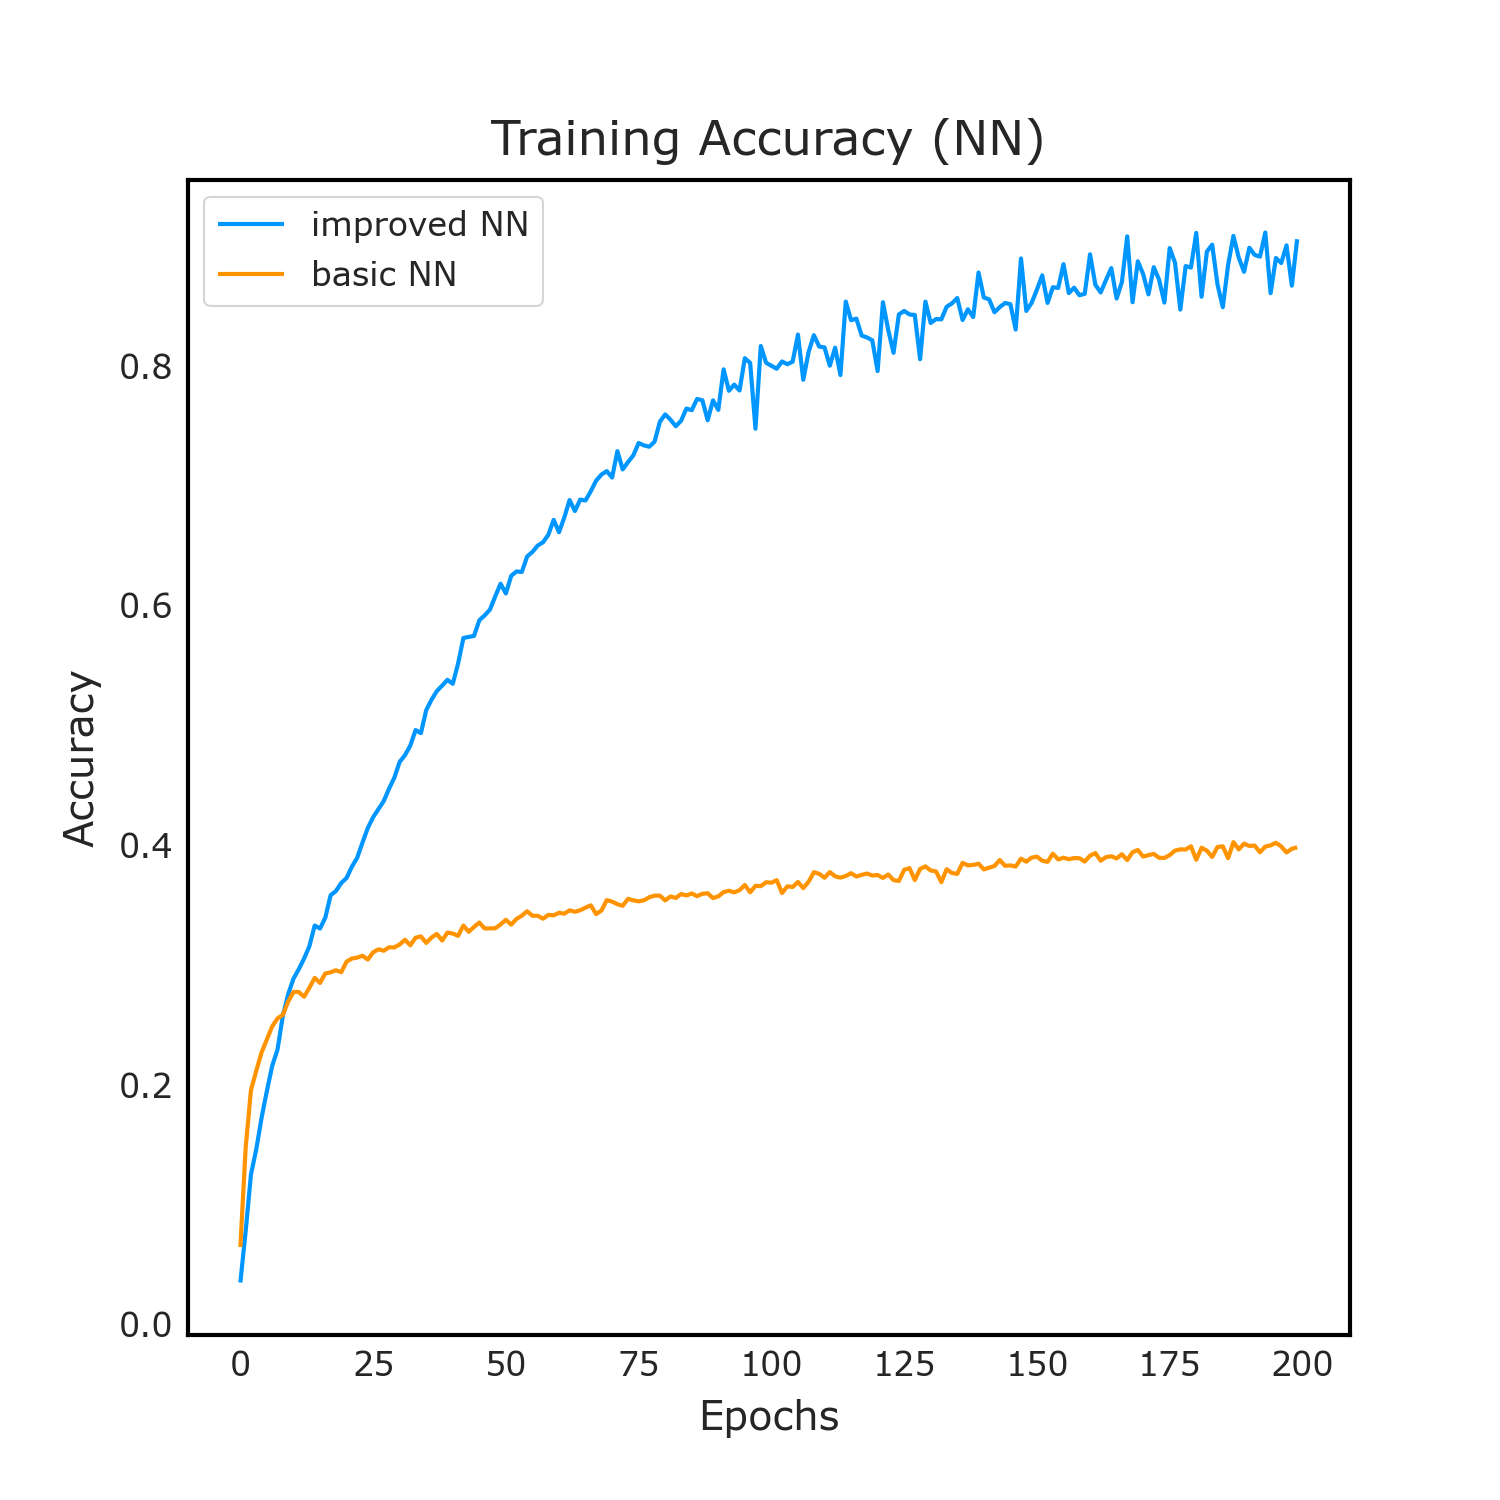
\includegraphics[width=\linewidth]{figs/train_accuracy.png}
        \caption{Training Accuracy per Epoch plot for Neural network}
        \label{fig:accuracy}
    \end{subfigure}%
    \begin{subfigure}{0.5\textwidth}
        \centering
        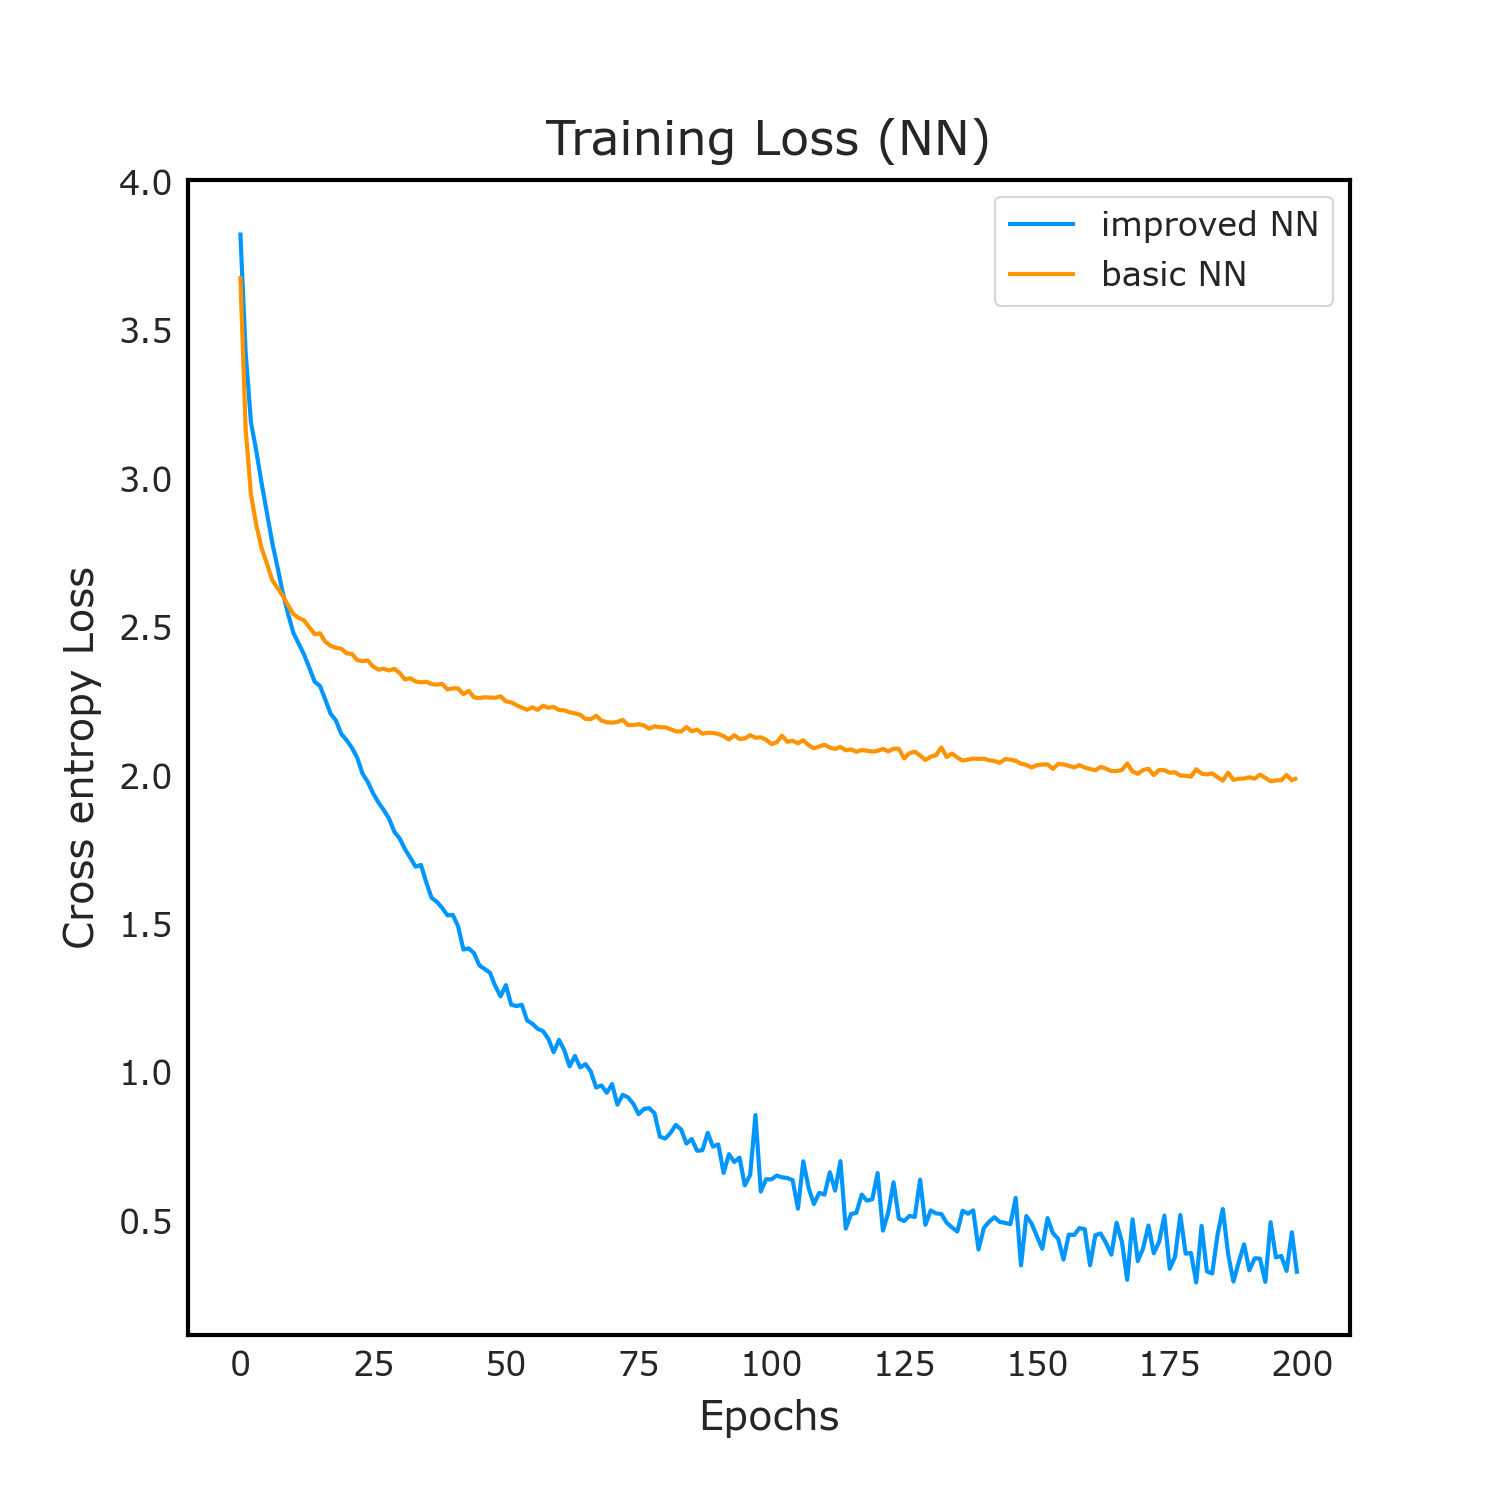
\includegraphics[width=\linewidth]{figs/train_loss1.png}
        \caption{Training Loss per Epoch plot for Neural Network}
        \label{fig:loss}
    \end{subfigure}
    \caption{Combined Figures}
    \label{fig:combined}
\end{figure}

\begin{figure}[h]
    \begin{subfigure}{0.5\textwidth}
        \centering
        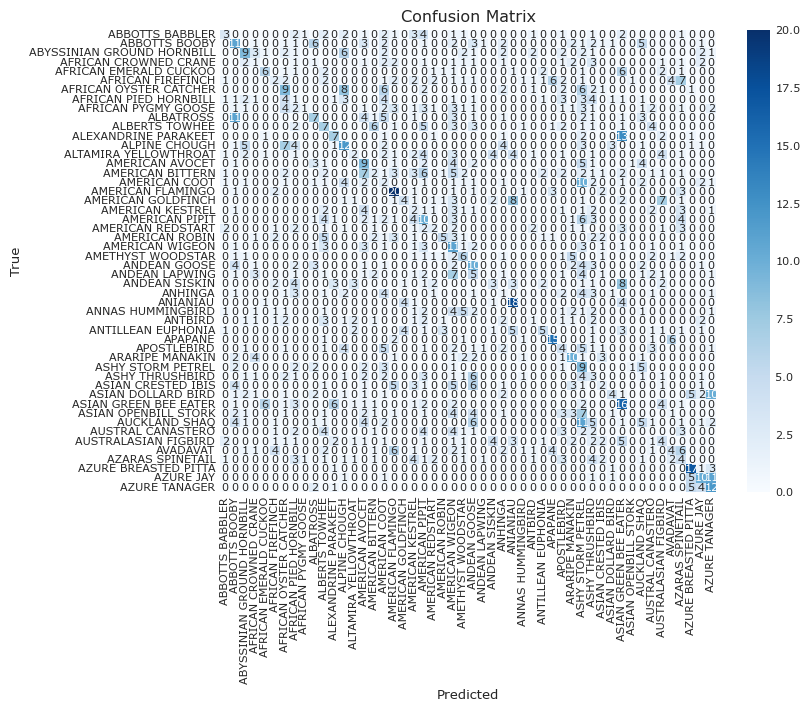
\includegraphics[width=\linewidth]{figs/matrix_baseline.png}
        \caption{Confusion matrix basic neural network}
        \label{fig:confusion basic}
    \end{subfigure}%
    \begin{subfigure}{0.5\textwidth}
        \centering
        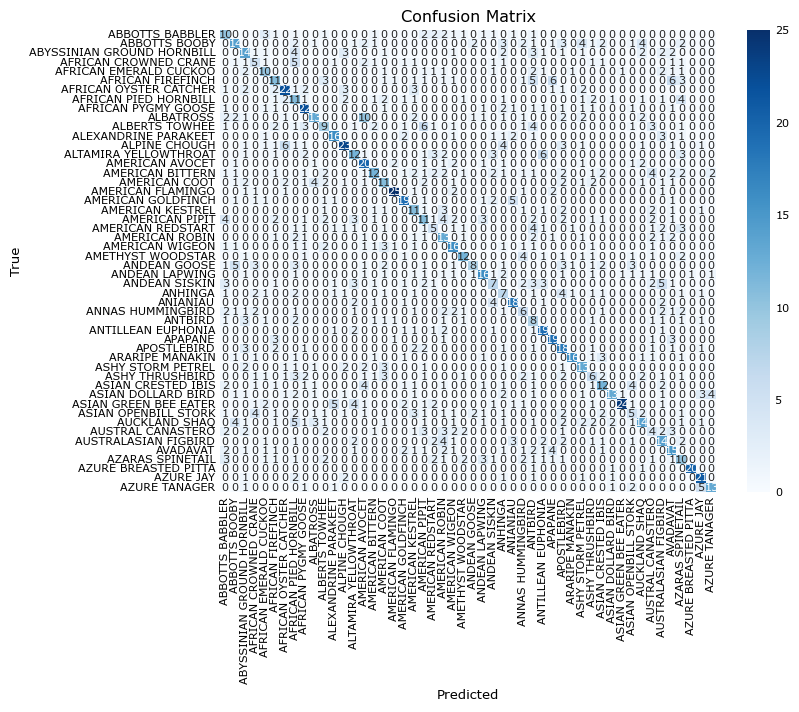
\includegraphics[width=\linewidth]{figs/matrix.png}
        \caption{Confusion matrix improved neural network}
        \label{fig:confusion improved}
    \end{subfigure}
    \caption{Combined Figures}
    \label{fig:combined}
\end{figure}

\section{Conclusion and Future Work}
Summarize your report and reiterate key points. Which algorithms were the highest- performing? Why do you think that some algorithms worked better than others? For future work, if you had more time, more team members, or more computational resources, what would you explore?

If we had more time and more team members, we would be able to work on the comparison between the different classes to see what the problem is for these classes of bird species. We can see if they really look alike of maybe are there some problem in the dataset with these pictures. For example we could also compare the AUC-PR for all different classes, this way we can easily see how well the model discriminates between all the different classes, and where there is much room for improvement. 

We could also improve the fully connected layers by implementing some convolutional layers because compared to the fully connected layers they are better at detecting spatial dimensions, which can be useful for images as these layers are able to detect some edges and textures. This is also visible in the ResNet50 which already uses convolutional layers. 

We could also add some dropout layers to the improved neural network \ref{fig:NN with 8 layers}. This way a random fraction of the input units is set to zero during training. This helps the model from relying too much on specific neurons and encourages the network to learn the more robust features. Also we could add batch normalization layers to the improved neural network \ref{fig:NN with 8 layers}. This way we could normalize the input by subtracting the batch mean and dividing by the batch standard deviation. This is done on each feature independently. 
\section{Contributions}
The contributions section is not included in the 6 page limit. This section should describe what each team member worked on and contributed to the project.

Joren Mangelschots: I worked on the neural network methods. I started by using the code of the exercise session about "neural networks for multiclass classification". I used the .csv file provided by the dataset from which I get the image path, then I transform the image to an array which i store in my X variable, as my Y I store the labels of the corresponding species of birds. I first used the model of the exercise session which adapted so the output layer contains 50 neurons and the first two connected layers contain 64 neurons. I added a flatten layer before the connected layers to have a 1D array to insert in my connected layers. 

To improve the changed model I increased the amount of layers and the amount of neurons to increase the complexity of the model. This way I would have more trainable parameters. Then i compared both of these models. I changed the learning rate to find the best value for me and also played around with some batch sizes. The learning rate for the end result is 0.001 for both models, and the batch size is 32 for both. With these values I got the best result. I kept the improved model only with more layers and neurons and without any dropout layers or other techniques to prevent overfitting. To really be able to display the result of adding more layers and more neurons to your model. 

\bibliographystyle{plainnat} % Example style
\bibliography{citations.bib} % Replace with your .bib file's name

\end{document}